\documentclass[letterpaper, 12pt]{math}

\usepackage{pgfplots}

\pgfplotsset{compat=1.10}
\usepgfplotslibrary{fillbetween}
\usetikzlibrary{patterns}
\usetikzlibrary{calc}

\geometry{letterpaper, margin=1in}

\title{Section 6.2}
\author{Alvin Lin}
\date{Calculus II: August 2016 - December 2016}

\begin{document}

\maketitle

\section*{Problem 8}
\[ y = 6-x^{2} \quad y = 2 \]
\begin{center}
  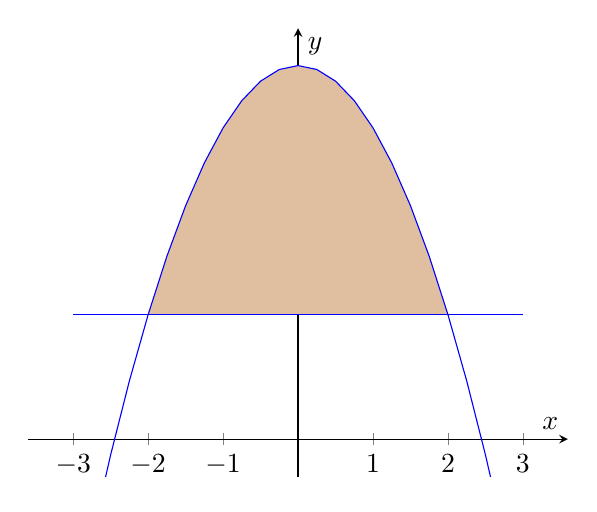
\begin{tikzpicture}
    \begin{axis}[axis lines=middle,
                 xlabel=\(x\), ylabel=\(y\),
                 ymin=0,
                 enlargelimits,
                 ytick=\empty]
      \addplot[name path=F, blue, domain={-3:3}]{6-x^2};
      \addplot[name path=G, blue, domain={-3:3}]{2};
      \addplot[color=brown!50] fill between [
               of=F and G, soft clip={domain=-2:2}];
    \end{axis}
  \end{tikzpicture}
\end{center}
\[ V = \int{A\diff{x}} \]
\[ V = \int{\pi(R1)^{2}-(R2)^{2}\diff{x}} \]
\[ V = \pi\int_{-2}^{2}{(6-x^{2})^{2}-(2)^{2}\diff{x}} \]
\[ V = \pi\int_{-2}^{2}{36-12x^{2}+x^{4}-4\diff{x}} \]
\[ V = \pi\int_{-2}^{2}{x^{4}-12x^{2}+32\diff{x}} \]
\[ V = \pi\bigg[\frac{x^{5}}{5}-\frac{12x^{3}}{3}+32x\bigg]_{-2}^{2} \]
\[ V = \frac{384\pi}{5} \]

\section*{Problem 11}
\[ y = x^{2} \quad x = y^{2} \]
\begin{center}
  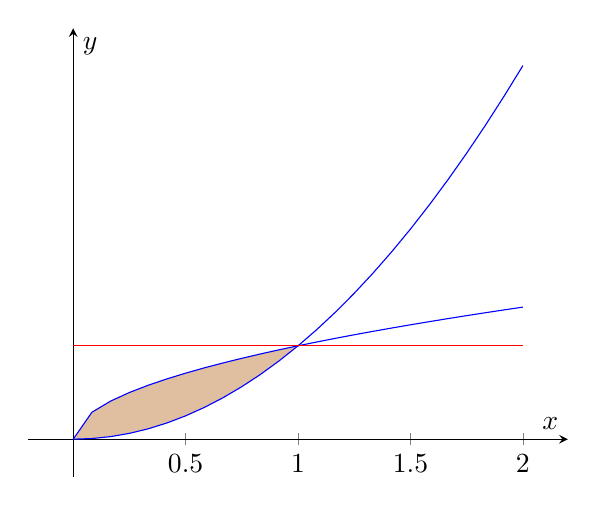
\begin{tikzpicture}
    \begin{axis}[axis lines=middle,
                 xlabel=\(x\), ylabel=\(y\),
                 enlargelimits,
                 ytick=\empty]
      \addplot[name path=F, blue, domain={0:2}]{x^2};
      \addplot[name path=G, blue, domain={0:2}]{sqrt(x)};
      \addplot[name path=A, red] coordinates {(0, 1) (2, 1)};
      \addplot[color=brown!50] fill between [
               of=F and G, soft clip={domain=0:1}];
    \end{axis}
  \end{tikzpicture}
\end{center}
\[ V = \int{A\diff{x}} \]
\[ V = \int{\pi(R1)^{2}-(R2)^{2}\diff{x}} \]
\[ V = \pi\int_{0}^{1}{(1-x^{2})^{2}-(1-\sqrt{x})^{2}\diff{x}} \]
\[ V = \pi\int_{0}^{1}{(1-2x^{2}+x^{4})-(1-2\sqrt{x}+x)\diff{x}} \]
\[ V = \pi\int_{0}^{1}{x^{4}-2x^{2}-x+2\sqrt{x}\diff{x}} \]
\[ V = \pi\bigg[\frac{x^{5}}{5}-\frac{2x^{3}}{3}-
       \frac{x^{2}}{2}+\frac{4x^{3/2}}{3}\bigg]_{0}^{1} \]
\[ V = \frac{11\pi}{30} \]

\section*{Problem 17}
\[ x = y^{2} \quad x = 1-y^{2} \]
\begin{center}
  about \( x = 3 \).
\end{center}
\[ V = \int{A\diff{y}} \]
\[ V = \int{\pi(R1)^{2}-(R2)^{2}\diff{y}} \]
\[ V = \pi\int_{-2\sqrt{2}}^{2\sqrt{2}}
       {(3-y^{2})^{2}-(3-(1-y^{2}))^{2}\diff{y}} \]
\[ V = \pi\int_{-2\sqrt{2}}^{2\sqrt{2}}
       {(9-6y^{2}+y^{4})-(y^{4}+4y^{2}+4)^{2}\diff{y}} \]
\[ V = \pi\int_{-2\sqrt{2}}^{2\sqrt{2}}{5-10y^{2}\diff{y}} \]
\[ V = \pi\bigg[10y-\frac{10y^{3}}{3}\bigg]_{-2\sqrt{2}}^{2\sqrt{2}} \]
\[ V = \frac{10\pi\sqrt{2}}{3} \]

\section*{Problem 29}
\[ x = 1-y^{2} \quad x=1-y \]
\[ V = \int{A\diff{y}} \]
\[ V = \int{\pi(R1)^{2}-(R2)^{2}\diff{y}} \]
\[ V = \pi\int_{0}^{1}{(1-y^{2})^{2}-(1-y)^{2}\diff{y}} \]
\[ V = \pi\int_{0}^{1}{1-2y^{4}+y^{8}-(1-2y+y^{2})diff{y}} \]
\[ V = \pi\int_{0}^{1}{y^{8}-2y^{4}-y^{2}+2y\diff{y}} \]
\[ V = \pi\bigg[\frac{y^{9}}{9}-\frac{2y^{5}}{5}-
       \frac{y^{3}}{3}-\frac{2y^{2}}{2}\bigg]_{0}^{1} \]
\[ V = \frac{17\pi}{45} \]

\section*{Problem 55}
\[ \frac{x^{2}}{2}+\frac{y^{2}}{9} = 1 \]
\[ y = \sqrt{36-9x^{2}} \]
\[ V = \int{A\diff{x}} \]
\[ V = \int{\pi r^{2}\diff{x}} \]
\[ V = \pi\int_{-2}^{2}{(\sqrt{36-9x^{2}})^{2}\diff{x}} \]
\[ V = \pi\int_{-2}^{2}{36-9x^{2}\diff{x}} \]
\[ V = \pi\bigg[36x-\frac{9x^{3}}{3}\bigg]_{-2}^{2} \]
\[ V = 24\pi \]

\begin{center}
  If you have any questions, comments, or concerns, please contact me at
  alvin@omgimanerd.tech
\end{center}

\end{document}
